\documentclass[fleqn]{beamer}
\usepackage{xcolor}
\usepackage{ctex}
\usepackage{slide}
\definecolor{Green}{RGB}{0,100,0}
\usepackage{t1enc}
\usepackage{setspace}
\usepackage{hyperref}
\usepackage{lmodern}
\usepackage{amsmath}
\setcounter{framenumber}{0}
\title{
The impact of daily diet and exercise on weight
}
\author{
    \href{mailto: korenson@cs.ccu.edu.tw}{Ren-Song Ko}, \href{mailto: wisleyqqq0630@alum.ccu.edu.tw}{Wen-Shou Hsu}, and  \href{mailto: stchi111u@cs.ccu.edu.tw}{Tzu-Chi Hsiao}
}
\date{}
\begin{document}
\begin{frame}
  \titlepage
  \begin{center}
  Official website is available \href{https://tomtchsiao.github.io/project/}{here}. \\
  Source code is available \href{https://tomtchsiao.github.io/project/下載/index.html}{here}.
\end{center}
\begin{figure}[h]
    \centering

\includegraphics[width=0.10\textwidth]{logo.png}
\end{figure}
\begin{center}
  Floor One, Innovation Building \\
  National Chung Cheng University, Chiayi county, Taiwan
\end{center}
\end{frame}
\begin{frame}
\frametitle{Outline}
\begin{itemize}
        \item Introduction
        \vspace{0.15 cm}
        \item Tools for develop model
        \vspace{0.15 cm}
        \item Results
        \vspace{0.15 cm}
        \item Conclusion
        \vspace{0.15 cm}
\end{itemize}
\end{frame}
\begin{frame}
\frametitle{Outline}
\begin{itemize}
        \item Introduction
        \vspace{0.15 cm}
        \item \textcolor{gray}{Tools for develop model}
        \vspace{0.15 cm}
        \item \textcolor{gray}{Results}
        \vspace{0.15 cm}
        \item \textcolor{gray}{Conclusion}
        \vspace{0.15 cm}
\end{itemize}
\end{frame}
\begin{frame}
\frametitle{Introduction}
\begin{itemize}
    \item People emphasize their health and strengthen it by exercising at the gym, in the park, or even at home.
    \vspace{0.15 cm}
    \item We aim to establish a website to help them check whether their \alert{healthy} is normal.
    \vspace{0.15 cm}
    \item Given their \textcolor{blue}{age, gender, height, weight, eating habits, activity level, goal, daily calories} and \textcolor{blue}{After days}. 
    \vspace{0.15 cm}
    \item Displays result with suggestions and amounts of each nutrient in histogram.
    \vspace{0.15 cm}
\end{itemize}
\end{frame}
\begin{frame}
\frametitle{Outline}
\begin{itemize}
        \item \textcolor{gray}{Introduction}
        \vspace{0.15 cm}
        \item Tools for develop model
        \vspace{0.15 cm}
        \item \textcolor{gray}{Results}
        \vspace{0.15 cm}
        \item \textcolor{gray}{Conclusion}
        \vspace{0.15 cm}
\end{itemize}
\end{frame}
\begin{frame}
\frametitle{Tools for develop model}
\begin{itemize}
    \item Programming Language: Python, HTML, CSS \\
    \vspace{0.15 cm}
    \item Data transmitting: Flask \\
    \vspace{0.15 cm}
    \item Aesthetic: JavaScript \vspace{0.15 cm}
\end{itemize}
\end{frame}
\begin{frame}
\frametitle{Outline}
\begin{itemize}
        \item \textcolor{gray}{Introduction}
        \vspace{0.15 cm}
        \item \textcolor{gray}{Tools for develop model}
        \vspace{0.15 cm}
        \item Results
        \vspace{0.15 cm}
        \item \textcolor{gray}{ Conclusion}
        \vspace{0.15 cm}
\end{itemize}
\end{frame}
\begin{frame}
\frametitle{Results}
     \begin{minipage}[t]{0.48\textwidth}
         \setbeamercolor{block title}{bg=red,fg=white}
         \setbeamerfont{block title}{size=\small}
         \setbeamerfont{block body}{size=\small}
        \begin{block}{Our anticipate}
         \setbeamercolor{itemize item}{fg=red}
            \begin{itemize}
                \item Accurately calculate the actual weight using a series of indexes, such as BMR, TDEE. \\
                \item Provide a histogram to show the amounts of each nutrient. 
            \end{itemize}
        \end{block}
    \end{minipage}%
    \hfill
    \begin{minipage}[t]{0.48\textwidth}
        \setbeamerfont{block title}{size=\normalsize}
        \setbeamerfont{block body}{size=\normalsize}
        \setbeamercolor{block title}{bg=Green,fg=white}
        \begin{block}{Our model anticipate}
            \begin{itemize}
            \setbeamercolor{itemize item}{fg=Green}
                \item Provide suggestion, different histograms for each nutrient.
            \end{itemize}
        \end{block}
\end{minipage}
\end{frame}
\begin{frame}{Results (Continued)}
\begin{figure}[h]
    \centering
    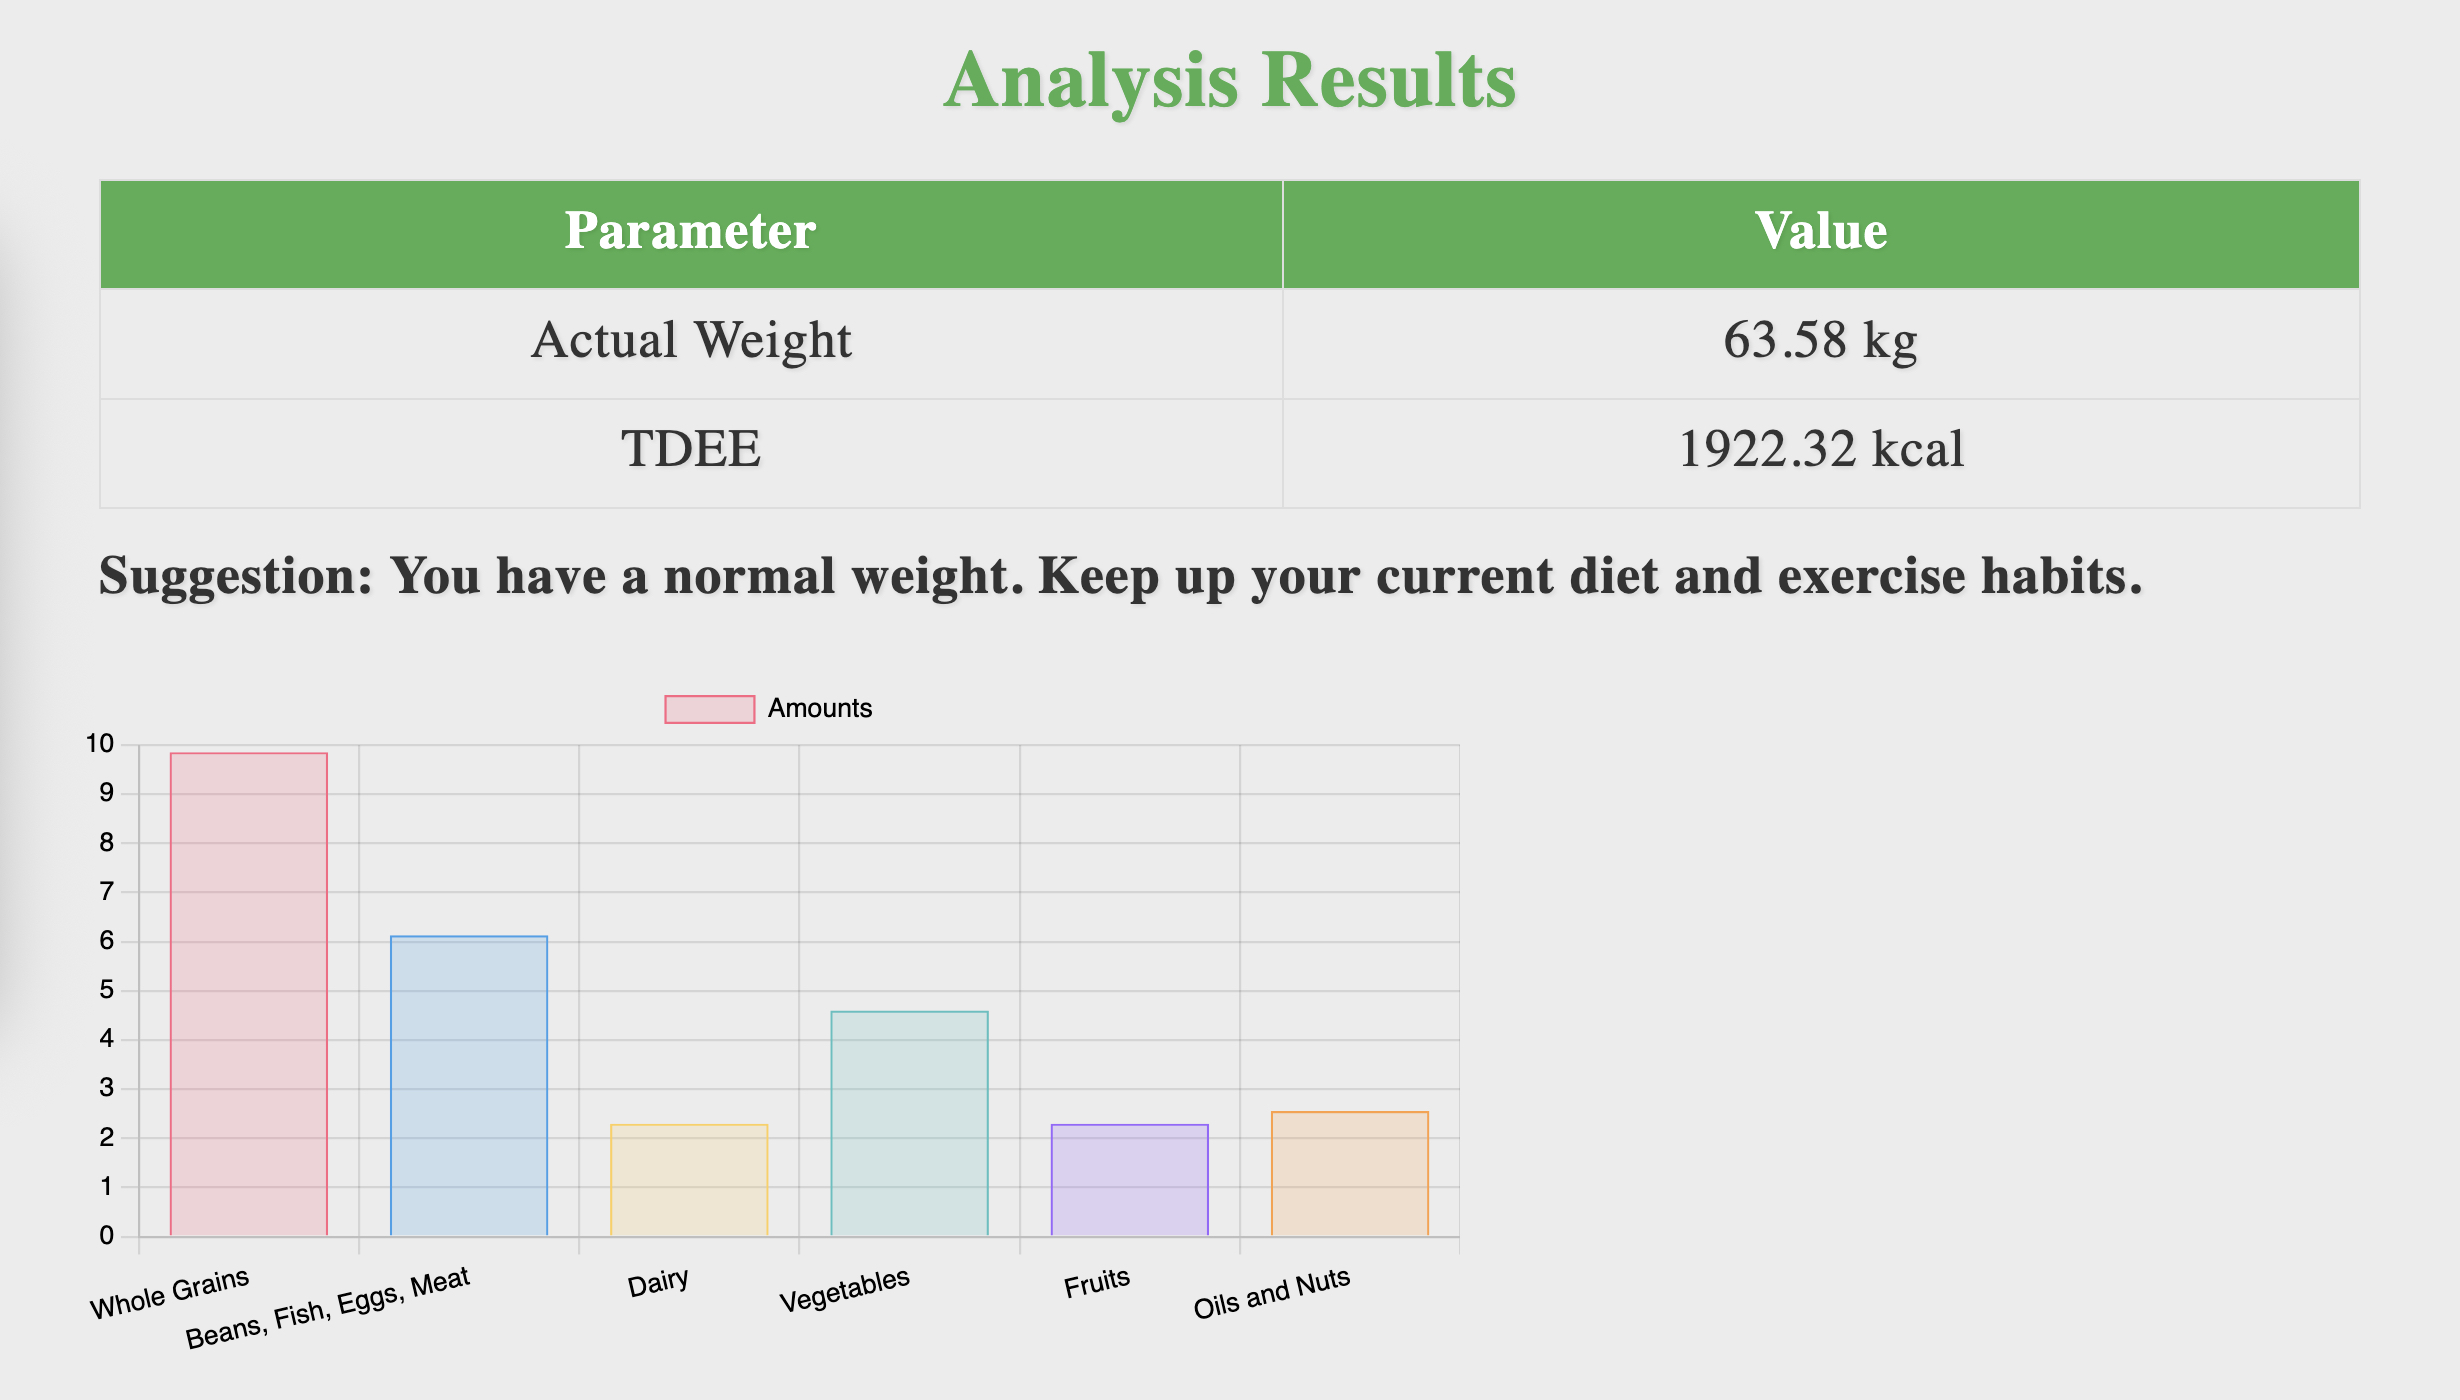
\includegraphics[width=\textwidth]{Example.png}
\end{figure}
    \centering
    Figure I. Results of entering data.
\end{frame}
\begin{frame}{Results (Continued)}
\vspace{1.5cm}
\sloppy
\renewcommand{\arraystretch}{1.5}
\centering
\begin{tabular}{|c|c|c|c|c|}
\hline
\textbf{Sedentary} & \textbf{Light} & \textbf{Moderate} & \textbf{Active} & \textbf{Very active} \\
\hline
1.2 & 1.375 & 1.55 & 1.725 & 1.9 \\
\hline
\end{tabular}
\vspace{0.5cm} 
\\
Table I. Consume calories from the exercise. 
\vspace{1cm} 
\\
\begin{tabular}{|c|c|c|c|}
\hline
\textbf{Vegetarian} & \textbf{Meat} & \textbf{Lacto ovo vegetarian} & \textbf{Balanced} \\
\hline
1800 & 2500 & 2200 & 2000 \\
\hline
\end{tabular}
\vspace{0.5cm} 
\\
Table II. Consume calories from the daily diet. 
\vspace{1cm} 
\\
\end{frame}
\begin{frame}{Results (Continued)}
\sloppy
\begin{align*}
    \text{Male's BMR} &= (9.99 \times \text{weight}) + (6.25 \times \text{height}) \\
    &\quad - (4.92 \times \text{age}) + (166 \times \text{gender} - 161) \\
    \text{Female's BMR} &= (9.99 \times \text{weight}) + (6.25 \times \text{height}) \\
    &\quad - (4.92 \times \text{age}) + (166 \times \text{gender} - 161)
    \end{align*}
\end{frame}
\begin{frame}{Results (Continued)}
\begin{align*}
\text{Each day} = \text{BMR} \times \text{Activity}
\end{align*}
\begin{align*}
\text{Intake} = \text{Daily diet type}
\end{align*}
\begin{align*}
\text{Calorie deficit} = \text{Intake} - \text{Calories per day}
\end{align*}
\begin{align*}
\text{Weight changes} = \frac{\text{Calorie deficit}}{7700} 
\end{align*}
\begin{align*}
    \text{Actual weight}= \text{Weight} + \text{Weight changes} \times \text{After days}
    \end{align*}
\begin{align*}
\text{BMI} = \frac{\text{Weight}}{\text{Height}^2}
\end{align*}
\end{frame}
\begin{frame}
\frametitle{Outline}
\begin{itemize}
        \item \textcolor{gray}{Introduction}
        \vspace{0.15 cm}
        \item \textcolor{gray}{Tools for develop model}
        \vspace{0.15 cm}
        \item \textcolor{gray}{Results}
        \vspace{0.15 cm}
        \item Conclusion
        \vspace{0.15 cm}
\end{itemize}
\end{frame}
\begin{frame}
\frametitle{Conclusion}
    \begin{itemize}
        \vspace{0.15 cm}
        \item Using precise tools to calculate the actual weight, ensuring that users receive accurate and reliable measurements for better health management.
        \vspace{0.15 cm}
        \item Providing accurate options for computation, allowing users to input various parameters and receive tailored recommendations based on their unique needs.
        \vspace{0.15 cm}
        \item We learned fundamental front-end and back-end development, including figure display using JavaScript and Python, to develop an application that seamlessly integrates user data and visualizes results effectively.
    \end{itemize}
\end{frame}
\begin{frame}{Acknowledgment}
\begin{block}{}
\normalsize
\setbeamerfont{block title}{size=\normalsize}
\setbeamerfont{block body}{size=\normalsize}
\setbeamercolor{itemize item}{fg=Green}
\begin{itemize}
    \setbeamerfont{itemize}{size=\small}
    \item Ren-Song Ko
    \item Wen-Shuo Hsu
    \item Tzu-Chi Hsiao
\end{itemize}
\end{block}
\vspace{1.5 cm}
\begin{block}{}
\normalsize
    \setbeamerfont{block title}{size=\normalsize}
    \setbeamerfont{block body}{size=\normalsize}
    \begin{center}
    \setbeamerfont{itemize}{size=\small}
    \textcolor{purple}{Thank you for listening! We wish you a pleasant day.}
    \end{center}
    \end{block}
\end{frame}
\end{document}